\subsection{General Overview} \label{arch:general Overview}
In this section, we will look at the architecture of Medchain system. We first begin by looking at the requirements that our software solution should be able to fulfil. Then, we discuss how our solution meets its requirements and objectives. 

\subsection{Requirements} \label{arch:requirements}
Medchain aims to offer distributed identity and access management mechanisms for (medical) data sharing systems. However, the main goal of this project is to apply Medchain for a specific medical data system called MedCo described in Section \ref{background:medco}. To achieve this, Medchain has to fulfil the following tasks and requirements:
\begin{enumerate}
    \item Offer its services in a distributed manner 
    \item Offer access management and user authentication 
    \item Authorize users and queries
    \item Enable auditability by recording a full history of queries in blockchain
    \item Work seamlessly with MedCo
\end{enumerate}
In the following sections, we study how each of the above-mentioned requirements are fulfilled in Medchain. 

\subsubsection{Distributed Services in Medchain} \label{arch:distributed}
As it was mentioned in the previous section, the first goal of Medchain is to offer services in a distributed manner. To achieve this, we used conodes. Conodes make the foundation for Medchain. They support distributed protocols and services provided by the \href{https://github.com/dedis/onet/blob/master/README.md}{onet} library (a part of Cothority project developed by DEDIS at EPFL). Consequently, Medchain is able to offer access management in a distributed manner. 

\subsubsection{Authentication in Medchain}\label{arch:authentication}
The goal of authentication is to verify the identity of the user who wants to access a specific resource such as data. In Medchain, user authentication is delegated to Keycloak \cite{keycloak:2019} which is the identity provider. This means that once Medchain receives a query from a user, we can simply assume that he/she is already authenticated and his/her identity and the user identity is submitted to Medchain as part of the query. We will discuss this in more details in Section \ref{arch:flow}, where the flow of query in Medchain is described comprehensively.

\subsubsection{Authorization in Medchain}\label{arch:authorization}
The goal of authorization is to control the user access to resources (e.g., data) based on his/her access level. In Medchain, we use Darcs (described in Section \ref{background:darc}) to enable user authorization and access management. 


\subsubsection{Auditability of Medchain} \label{arch:audit}
Auditability in Medchain means that there should be a mechanism in place so that the users can track all the queries submitted to Medchain server. Consequently, trace of any data misuse, data abuse, security/privacy breach, etc. can be found and mitigated later. 

In Medchain, we use blockchains to offer auditability. The blockchain framework we used in Medchain is ByzCoin (see Section \ref{background:byzcoin}). Every query sent by the user and its status, whether it is authorized or rejected, is recorded in the immutable ledger. 

\subsection{Medchain High-level View} \label{arch:high-level view}

Figure \ref{fig:medchain_node} shows the full architecture of a Medchain node. Every Medchain node is a conode and it contains three important building blocks. Below you can find more about each of these building blocks and their purpose:
\begin{itemize}
    \item \textbf{Smart contract}: offers user API and distributed access management 
    \item \textbf{Darcs}: manage user's access to resources 
    \item \textbf{Blockchain}: auditability 
\end{itemize}

Additionally, every Medchain node has 1 or more projects in it. A project is an abstract notion that wraps around a specific data resource and restricts access to it. Implementation-wise, every project is, in fact, a Darc that controls the access rights concerning a specific database.

\begin{figure}[ht] 
        \centering 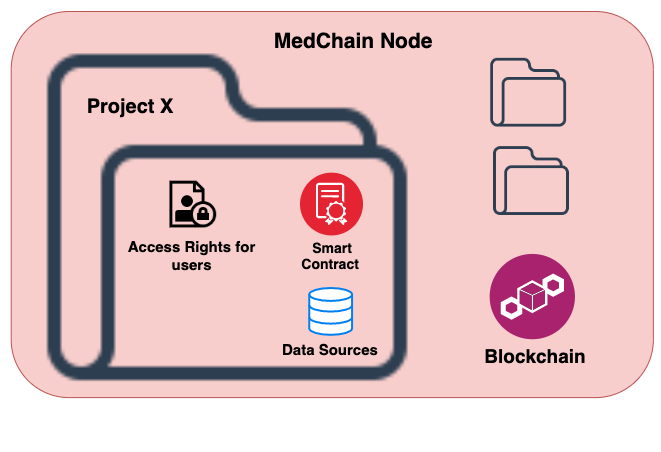
\includegraphics[width=0.7\columnwidth]{Images/medchain_node.png}
        \caption{\label{fig:medchain_node} 
         The structure and building blocks of a Medchain node.
        }
\end{figure}

\subsection{Flow of Queries in Medchain}\label{arch:flow}
Figure \ref{fig:medchain_workflow} illustrates the full architecture of Medchain and its detailed workflow starting from query creation and submission by the client until the query is executed. 

In this figure, there are three hospitals each running their own local Medchain server (conode). Now, focusing only on the user at Hospital 1, we describe the enumerated steps in Figure \ref{fig:medchain_workflow} as following:

\begin{enumerate}
    \item \textbf{User Login}: Client receives the token (i.e., its identity) from Keycloak.
    
    \item \textbf{Query Creation \& Submission}: User spawns a query. The query is submitted to MedCo-connector (i.e., service provider). 
    
    \item \textbf{User Authentication}: MedCo-connector verifies the token (i.e., the identity) of the user. 
    
    \item \textbf{Submission of Query To Medchain}: MedCo-connector sends the query that contains the user’s identity (i.e., part of the token) to Medchain server. The query that Medchain receives has a structure as below:
    Query's structure is as below:
    \begin{verbatim}
        {ID:<Query ID>,Status:<Query Status>}
    \end{verbatim}
The query itself has the following format:
   \begin{verbatim}
       <user_id>:<databaseX>:<type of query>
   \end{verbatim}
   Where \texttt{<user\_id>} is part of the user's token provided by Keycloak, \texttt{<databaseX>} is the name of the database (i.e., the project) user is querying, and \texttt{<type of query>} is what the user is trying to access from the database which can be one of the below:
   \begin{itemize}
        \item \texttt{patient\_list}
        \item \texttt{count\_per\_site}
        \item \texttt{count\_per\_site\_obfuscated}
        \item \texttt{count\_per\_site\_shuffled}
        \item \texttt{count\_per\_site\_shuffled\_obfuscated}
        \item \texttt{count\_global}
        \item \texttt{count\_global\_obfuscated}
   \end{itemize}
   
   Finally, \texttt{Status} is the status of the query in Medchain and it could be: \texttt{"Submitted"}, \texttt{"Authorized"}, or \texttt{"Rejected"}.
   
    \item \textbf{Query Transaction Creation}: \label{workflow:step 5}
    Medchain creates a transaction to spawn a \texttt{Query} (i.e., an instance of \texttt{queryContract}) and signs it. The transaction looks like below:
        \begin{verbatim}
CreateTransaction(byzcoin.Instruction{
    InstanceID:    byzcoin.NewInstanceID(<Project X Darc ID>),
    Spawn: &byzcoin.Spawn{
        ContractID: queryContract,
        Args: byzcoin.Arguments{
                {
                    Name:  <user_id>:<databaseX>:<type of query>,
                    Value: []byte("Submitted"),
                },
        },
})
        \end{verbatim}
        
    \item \textbf{Query Authorization}: The original Medchain node broadcasts the transaction proposal to the rest of the Medchain nodes in cothority network so that it is recorded in the ledger. Each Medchain server fetches the project Darc by the provided ID and checks if the query can be executed based on the identity of the user who submitted the query, what the query is, and the target project according to \texttt{Project X Darc} and the associated smart contract (i.e., \texttt{queryContract}).
    
    If a number of Medchain servers in the network are down and/or the responsible entities to accept or reject a query are not present (e.g., a manager at the hospital) at the time of transaction broadcast, the transaction execution is deferred until the threshold number of entities can react to it and either reject or accept it.  
    
    If the query is authorized by the Darc, and all Medchain servers approve it, the \texttt{Status} of the query is updated to \texttt{Authorized} and if it is rejected, the \texttt{Status} is set to \texttt{Rejected}. In any case, the query and the result of this stage is written to the ledger. 
    
    \item \textbf{Query Execution}: In the mean time, MedCo-connector is waiting for a reply from Medchain nodes. If the query is authorized, the query is directed to MedCo-connector in order for execution; otherwise, MedCo-connector receives a rejection message from Medchain. (In fact, MedCo-connector, i2b2 server, and MedCo-UnLynx all take part in query execution step, however, because the focus here is on Medchain, we overlook the details related to the query execution and only resort to high-level descriptions.) 
    
    \item \textbf{Commit Final Query Status To The Ledger}: After MedCo-connector executes the query, it submits the new query status (e.g., “Executed”) to Medchain server. Then, Medchain creates a transaction to update the status of the query to \texttt{Executed}. Finally, this transaction is added to the ledger. 

Starting from step \ref{workflow:step 5}, the query's \texttt{InstanceID} is preserved and using this \texttt{InstanceID}, we can keep track of the query and update its status accordingly. This is explained in more details in Section \ref{impl:darcs}.
    
\end{enumerate}
 
 
 \begin{figure}[htbp] 
        \centering 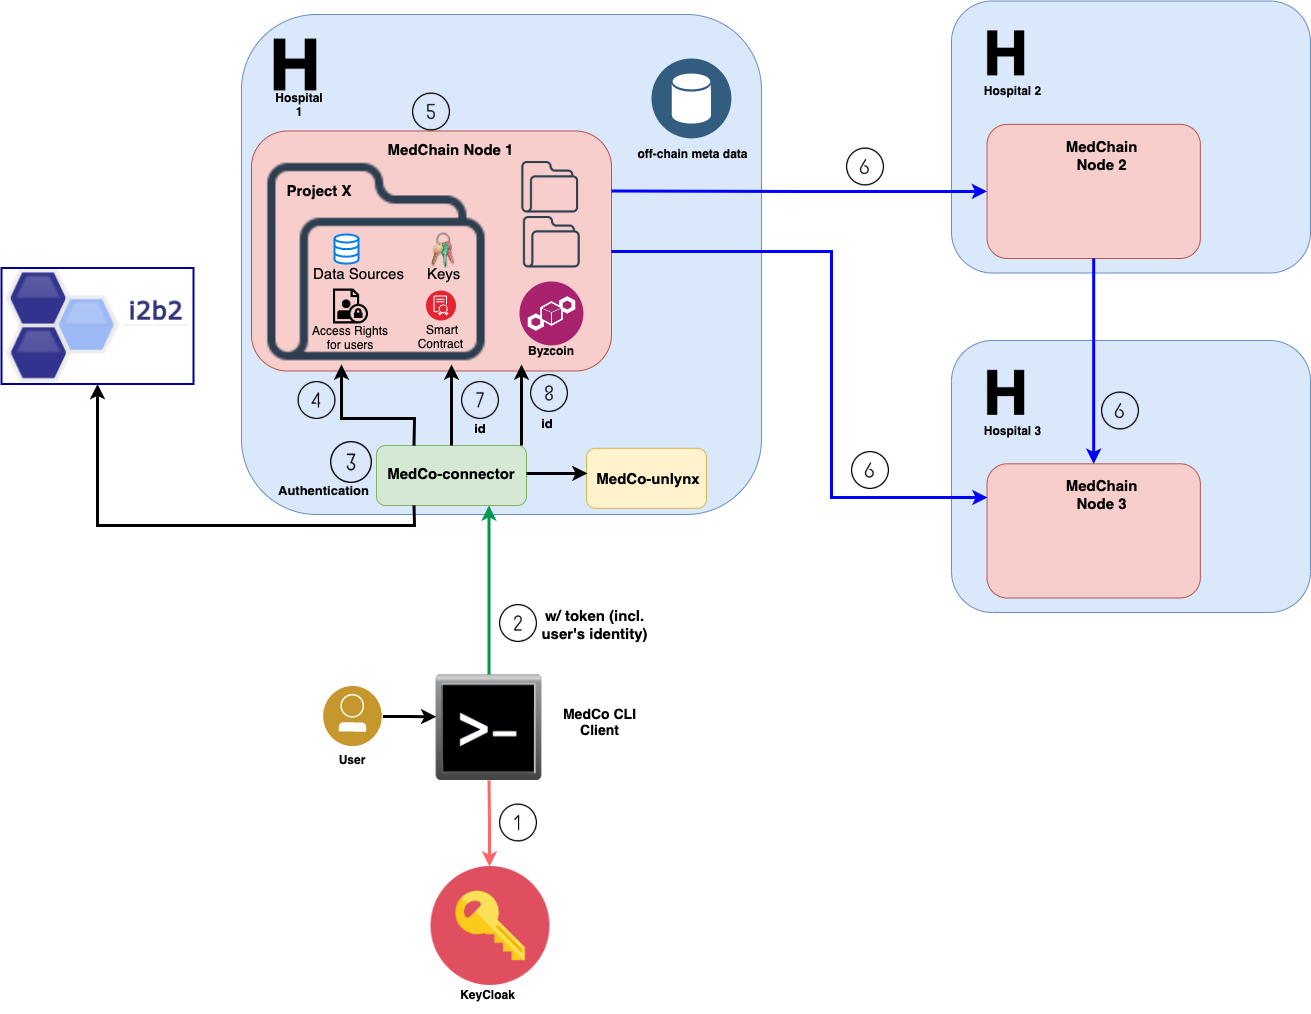
\includegraphics[width=1\columnwidth]{Images/medchain_msg.png}
        \caption{\label{fig:medchain_workflow} 
         Medchain architecture: workflow of queries in Medchain.
        }
\end{figure}
